\documentclass{beamer}
\usepackage{ctex}
\usepackage[export]{adjustbox}
\usepackage{listings}
\usepackage{xcolor}

\usetheme{focus}

\definecolor{codegreen}{RGB}{50 200 50}
\definecolor{codeblue}{RGB}{50 50 200}
\definecolor{codered}{RGB}{200 50 50}
\tikzset{
    global scale/.style={scale=#1,every node/.append style={scale=#1}},
    CC1/.style ={circle,minimum width = 30pt, minimum height =30pt, draw=black},
    CC2/.style ={circle,minimum width = 30pt, minimum height =30pt, draw=black, fill=blue!20},
    RA1/.style ={rectangle,minimum width = 30pt, minimum height =20pt, draw=black},
    RA2/.style ={rectangle,minimum width = 1cm, minimum height = 1cm, draw=black}
}

\title{算法分析与设计II}
\subtitle{2022-2023-2}
\date{Last Modified: 2023.1.16}
\institute{\vspace{2em} 数学与计算机学院 \\ 数据科学与大数据技术}
\titlegraphic{\vspace{5em} 
\includegraphics[scale=0.3]{fig/jlnu.pdf}}

\lstset{
    columns=flexible,       
    numbers=left,  
    numberstyle=\footnotesize\color{darkgray},  
    frame=shadowbox, 
    rulesepcolor= \color{gray}, 
    keywordstyle=\color{codeblue},         
    commentstyle=\color{codegreen},  
    stringstyle=\color{codered}, 
    showstringspaces=false,  
    xleftmargin=3em,
    xrightmargin=1em,              
    language=c++                           
}

\tikzset{
    CC1/.style ={
    circle,
    minimum width = 30pt, 
    minimum height =30pt, 
    draw=black
    }
}

\begin{document}
\frame{\titlepage}
\section{6. 高级数据结构}
\begin{frame}{6.1 并查集}
    \begin{itemize}
        \item \textcolor{blue}{不相交集合数据结构}(Disjoint Set) :将编号分别为$1…n$的$n$个对象划分为不相交集合,在每个集合中,选择其中某个元素$x$代表所在集合
        \item 基本操作:
        \begin{itemize}
            \item MAKE-SET(x) 	建立新的集合,唯一成员$x$
            \item UNION(x,y) 	将包含$x$和$y$的两个集合合并成一个新的集合
            \item FIND(x) 		返回指针,指向包含$x$的集合的\textcolor{blue}{“代表”}(representative)
        \end{itemize}
        \item 由于两个基本操作是\textcolor{blue}{UNION}(合并)和\textcolor{blue}{FIND}(查找),所以称为“并查集”
    \end{itemize}
\end{frame}
\begin{frame}{实现}
    \begin{itemize}
        \item 使用树的数据结构来表示并查集,在程序实现起来相对简单,森林中的每棵树作为一个集合,树的节点表示集合中的元素,树的根用来作为该集合的“代表”
        \begin{itemize}
            \item 查找操作相当于对树进行遍历,从某个节点沿着父节点指针找到这棵树的根节点
            \item 合并操作相当于两棵树合并成一棵树,两个节点位于两棵不同的树的时候,将一个节点所在树的根的父亲节点指向另一个节点所在树的根
        \end{itemize}
        \item 在具体程序实现中,使用一维数组p来实现,数组下标i表示每个节点,p[i]为指向其父节点的指针,即p[x]=y表示x的父节点为y
        \item p的初始值有两种设置方法,一种是均设为-1,另一种是令p[i]=i,两种方式在判断是否查找到树根有所不同,设成-1还有一个用处,可以用它来统计集合成员的数量
    \end{itemize}
\end{frame}
\begin{frame}{无向图的连通分量}
    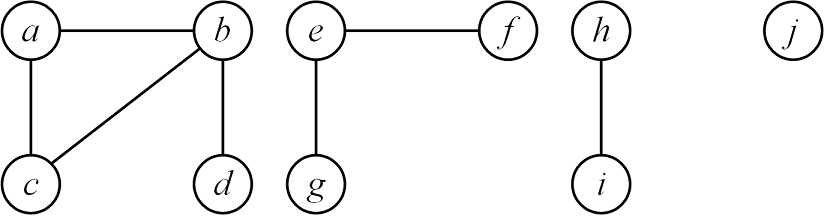
\includegraphics[width=0.7\textwidth,center]{fig/6-1.png}
    \begin{table}
        \begin{tabular}{c|c|c|c|c|c|c|c|c|c|c}
            边   & \multicolumn{10}{c}{构成的不相交集合} \\\hline
            初始     & \{a\}         & \{b\}   & \{c\}  & \{d\}  & \{e\}     & \{f\}  & \{g\}  & \{h\}   & \{i\}  & \{j\}  \\\hline
            (b,d)   & \{a\}         & \{b,d\} & \{c\}  & \{d\}  & \{e\}     & \{f\}  & \{g\}  & \{h\}   & \{i\}  & \{j\}   \\\hline
            (e,g)   & \{a\}         & \{b,d\} & \{c\}  &      & \{e,g\}   & \{f\}  &      & \{h\}   & \{i\}  & \{j\}   \\\hline
            (a,c)   & \{a,c\}        & \{b,d\} &      &      & \{e,g\}   & \{f\}  &      & \{h\}   & \{i\}  & \{j\}   \\\hline
            (h,i)   & \{a,c\}        & \{b,d\} &      &      & \{e,g\}   & \{f\}  &      & \{h,i\} &      & \{j\}   \\\hline
            (a,b)   & \{a,b,c,d\}    &       &      &      & \{e,g\}   & \{f\}  &      & \{h,i\} &      & \{j\}   \\\hline
            (e,f)   & \{a,b,c,d\}    &       &      &      & \{e,f,g\} &      &      & \{h,i\} &      & \{j\}   \\\hline
            (b,c)   & \{a,b,c,d\}    &       &      &      & \{e,f,g\} &      &      & \{h,i\} &      & \{j\}   \\\hline
        \end{tabular}
    \end{table}
\end{frame}
\begin{itemize}
    \item \textcolor{blue}{按秩合并}(union by rank)
    \begin{itemize}
        \item 增加一个Rank数组(初始值为0)来记录树的深度,也就是\textcolor{blue}{秩}
        \item 将秩较小的树的根指向秩较大的树的根
        \item 任意顺序的合并操作以后,包含$k$个节点的树的最大高度不超过$\log k$
    \end{itemize} 
\end{itemize}
\begin{lstlisting}
    void Union(int x,int y)  
    {   x = Find(x);
        y = Find(y);
        if(x==y) return;
        if(Rank[x] < Rank[y])
            p[x]=y;
        else {
            p[y]=x;
            if(Rank[x]==Rank[y])
                Rank[x]++;
        }
    }
\end{lstlisting}
    
\vspace*{3ex}
\begin{itemize}
    \item \textcolor{blue}{路径压缩}(path compression)
    \begin{itemize}
        \item 每次查找的时候,可以将查找路径上的节点修改成指向根节点,以便下次查找的时候速度更快
        \item 路径压缩的效果如图所示,(a)为压缩前,(b)为压缩后
    \end{itemize} 
\end{itemize}
\begin{columns}
    \column{0.6\textwidth}
    \begin{lstlisting}
    int Find(int x)
    {
        if(p[x] < 0)
            return x;
        p[x] = Find(p[x]);
        return p[x];
    }
    \end{lstlisting}
    \column{0.4\textwidth}
    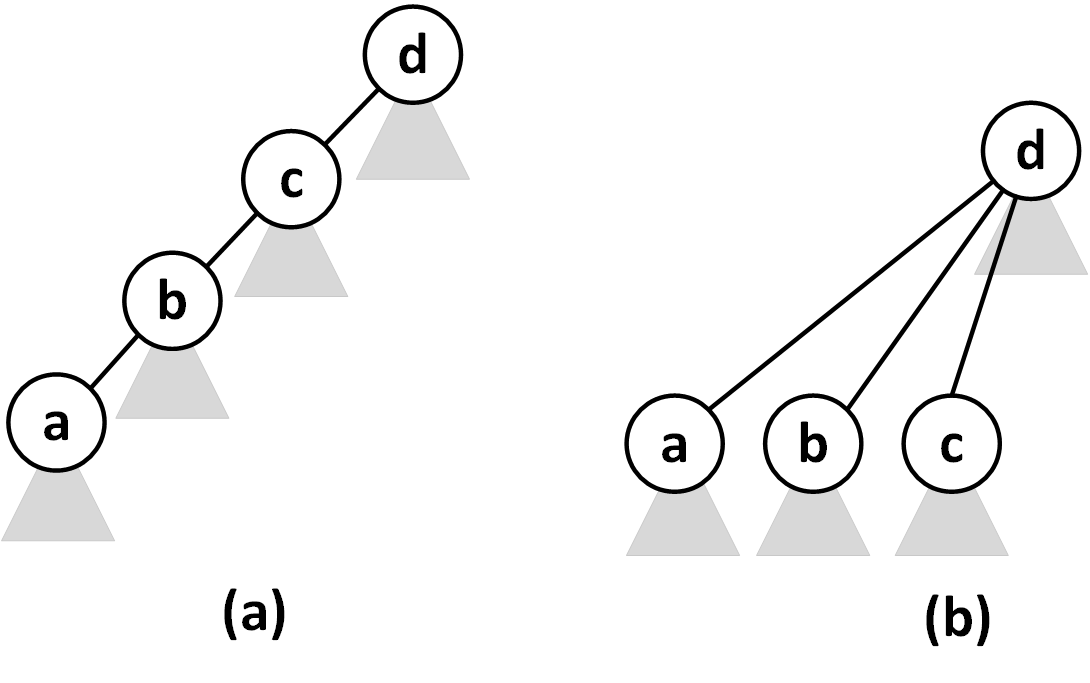
\includegraphics[width=\textwidth,right]{fig/6-2.png}
\end{columns}
\begin{frame}{2524 -- Ubiquitous Religions (poj.org)}
    \begin{itemize}
        \item $n$个学生信仰不同的宗教
        \vfill
        \item 给出$m$条信息,每条信息包含两个学生的编号,这两个学生信仰同一宗教
        \vfill
        \item 要求判断共有多少种宗教
    \end{itemize}
\end{frame}
\begin{frame}{6.2 线段树}
    \begin{itemize}
        \item \textcolor{blue}{线段树}(Segment tree) 使用二叉树的结构,每个节点表示一个包含起点和终点的区间,也可以看成是一个线段
        \vfill
        \item 线段树对区间信息进行存储,可以实现一些与区间计算有关的操作,例如区间最值问题、区间求和问题等,计算几何里面扫描线的操作也可以用线段树实现
        \vfill
        \item 由于线段树消耗大量存储空间,熟练掌握离散化处理方法十分重要
        \begin{block}{“在线” 与“离线”}
            \scriptsize{
                \quad 在程序设计过程中,如果开始时不需要知道所有输入,而是以序列的方式依次处理问题的算法,随着查询操作,数据也在实时变化,也称为“在线”查询,相应的算法称为\textcolor{blue}{在线算法},例如插入排序算法、贪心算法等\\
                \quad 相对的,开始时就需要知道问题的所有数据,每次查询操作时的数据保持不变,称为“离线”查询,相应的算法称为\textcolor{blue}{离线算法}。基于线段树的区间查询算法是离线查询,在多次查询的问题中能够提高效率}
        \end{block}
    \end{itemize}
\end{frame}
\begin{frame}{2182 -- Lost Cows (poj.org)}
    \begin{itemize}
        \item  $n$头牛编号为$1…n$,打乱顺序排成一列,除去队首的牛之外,给出每头牛在队列中前面编号比它小的牛的数量$k$,求队列中每头牛的编号
    \end{itemize}
    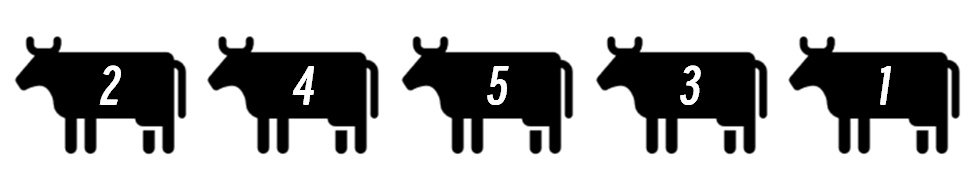
\includegraphics[width=0.8\textwidth,center]{fig/6-3.png}
    \begin{itemize}
        \item  维护一个线段树来解决该问题,创建一个线段树$T$,树中每个节点有3个属性$[p,r,n]$,分别代表线段左端点、线段右端点、左右端点之间节点的数量
    \end{itemize}
\end{frame}
\begin{frame}{构造线段树$(n=5)$}
    \begin{itemize}
        \item  从树根处依次比较:如果$k$小于等于左子树的$n$,则在左子树中继续查询;如果$k$大于左子树的$n$,则$k=k-n$,在右子树中继续查询;直到找到叶子节点($p=r$),此时的$p$即为要查询的编号
    \end{itemize}
    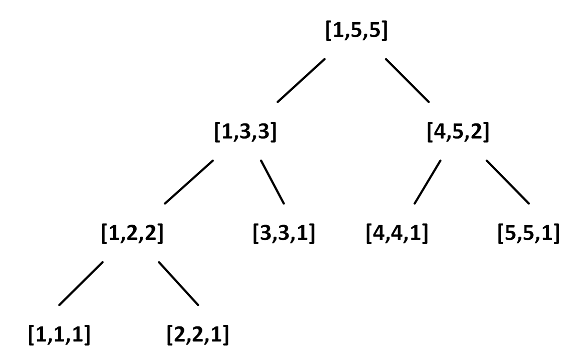
\includegraphics[width=0.8\textwidth,center]{fig/6-4.png}
\end{frame}
\begin{frame}{6.3 树状数组}
    \begin{itemize}
        \item \textcolor{blue}{树状数组}也称\textcolor{blue}{二元索引树}(Binary Indexed Tree)或\textcolor{blue}{Fenwick树}, 树状数组非常适合区间累计的计数与求和,尤其是多组查询,代码效率很高
        \item 与线段树相比,线段树可实现的功能更多,凡是树状数组能解决的问题,线段树同样可以解决
        \item 树状数组用一维数组C实现,每个元素代表不同区间(图中矩形横向范围)
        \begin{itemize}
            \item C[1]:[1-1],C[2]:[1-2],C[3]:[3-3],C[4]:[1-4],C[5]:[5-5],C[6]:[5-6],...
        \end{itemize}
    \end{itemize}
    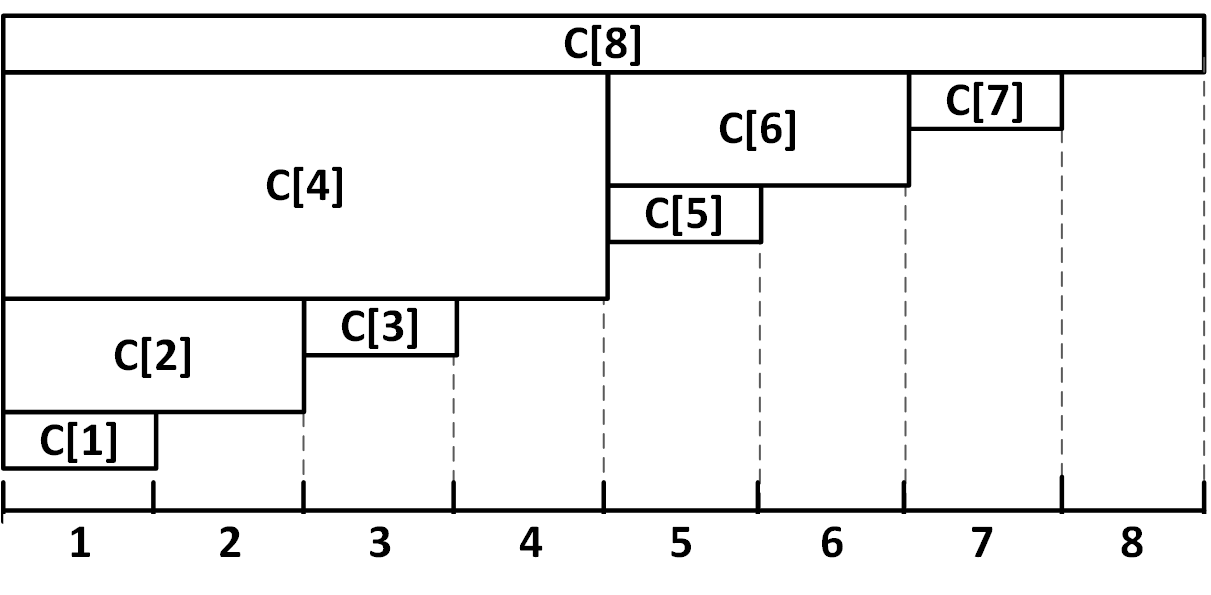
\includegraphics[width=0.7\textwidth,center]{fig/6-5.png}
\end{frame}
\begin{frame}{树状数组}
    \begin{itemize}
        \item 区间用下面方法确定:
        \begin{itemize}
            \item 将下标用二进制表示出来,然后看末位有几个0,设0的个数为$k$,则它代表的区间就向前推$2^k-1$
            \item 例如:$6=(110)_2$,$k=1$,向前推$2^1-1=1$,所以表示的区间为[5-6]
        \end{itemize}
        \item 树状数组两个基本操作:
        \begin{enumerate}[(1)]
            \item 更新/添加元素$x$:将$x$对应“列”的C值更新
            \begin{itemize}
                \item 例如:$x=1$,需要将$C[1],C[2],C[4],C[8]\ldots$都更新
                \item 计数:对应位置加1
                \item 求和:对应位置加$x$
            \end{itemize}
            \item 区间求和:将对应区间“行”的C值相加
            \begin{itemize}
                \item 对于$[1\ldots n]$区间求和,只需将对应“行”的C值相加,例如
                $$\sum [1\ldots 7]=C[4]+C[6]+C[7]$$ 
                \item 对于$[m\ldots n]$区间求和,只需$\sum [1\ldots n]$减去$\sum [1\ldots m-1]$,例如
                $$\sum[3\ldots 5]=\sum [1…5]-\sum [1…2]=C[4]+C[5]-C[2]$$
            \end{itemize}
        \end{enumerate}
    \end{itemize}
\end{frame}
\begin{frame}{lowbit}
    \begin{itemize}
        \item 计算公式:$lowbit(x)=x\&(-x)$,例如:$lowbit(6)$
        \begin{table}
            \begin{tabular}{r|c}
                十进制 & 二进制(32位int类型)                    \\\hline
                6   & \texttt{00000000000000000000000000000110} \\\hline
                -6  & \texttt{11111111111111111111111111111010}\\\hline
                \&  & \texttt{00000000000000000000000000000010} \\\hline
            \end{tabular}
        \end{table}
        \item 计算出来的$lowbit$值见下表
        \begin{table}
            \begin{tabular}{r|cccccccc}
                x         & 1    & 2    & 3    & 4    & 5    & 6    & 7    & 8 \\\hline
				lowbit(x) & 1    & 2    & 1    & 4    & 1    & 2    & 1    & 8 \\\hline
            \end{tabular}
        \end{table}
        \item 观察树状数组的两个基本操作可以发现,下标的变化值为上一个下标的$lowbit$值
        \begin{enumerate}[(1)]
            \item “更新”的列的下标变化,例如1对应列C的下标为{1,2,4,8,…},变化值为$lowbit(1),lowbit(2),lowbit(4),\ldots$ 
            \item “求和”的行的下标变化,例如[1-7]对应行C的下标为{7,6,4},变化值为$lowbit(7),lowbit(6)$            
        \end{enumerate}
    \end{itemize}
\end{frame}
\begin{frame}{2352 -- Stars (poj.org)}
    \begin{itemize}
        \item  给出$n$个星星的坐标$(x,y)$,按$y$递增,$y$相等$x$递增的次序
        \item 一颗星星的level定义为所有$x$和$y$均不大于该星星坐标的星星的总数,如图所示,编号1…5的星星的level分别为0,1,2,1,3
        \item 依次输出level为0…n-1的星星个数,level为0的有1个,level为1的有2个,依次类推,所以输出1,2,1,1,0
    \end{itemize}
    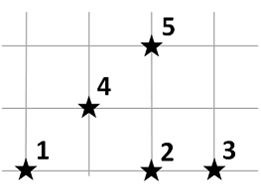
\includegraphics[width=0.4\textwidth,center]{fig/6-6.png}
    \begin{itemize}
        \item  本题中给出的星星坐标已经将$y$递增排序,统计每个星星$x$坐标之前有多少个星星即可,也就是每输入一个星星的坐标,level值就是[1…x-1]的累计值
    \end{itemize}
\end{frame}
\begin{frame}{6.4 二叉搜索树}
    \begin{itemize}
        \item  \textcolor{blue}{二叉搜索树}(BST, Binary search tree) 具有如下性质:
        \begin{enumerate}[(1)]
            \item root是二叉搜索树的节点,x是root节点的值
            \item 如果left是root左子树的节点,则left.x≤root.x
            \item 如果right是root右子树的节点,则right.x≥root.x
        \end{enumerate}
        \vfill
        \item 一般的二叉搜索树在最坏情况下,将长度为n的有序序列插入后,将变成一个长度为n的链表,查找效率降低
        \vfill
        \item 为了解决这个问题,产生了各种平衡树 ,常见的有\textcolor{blue}{AVL树} ,\textcolor{blue}{树堆}(Treap),\textcolor{blue}{伸展树}(Splay tree ),\textcolor{blue}{红黑树}(Red-black tree)等
    \end{itemize}
\end{frame}
\begin{frame}{2418 -- Hardwood Species (poj.org)}
    \begin{itemize}
        \item 给出一个单词列表,将这些单词去重之后按字典序排序,并计算出每个单词出现的次数在总单词数中的比例
        \vfill
        \item 使用二叉搜索树来存储单词和查找,树中每个节点包含左节点、右节点、单词、单词出现的次数这几个属性
        \vfill
        \item C++ STL中的关联容器map\footnote{\url{https://cplusplus.com/reference/map/map/}}就是使用二叉搜索树实现,map内部通过自建一棵红黑树,实现了数据的自动排序和查找
    \end{itemize}
\end{frame}
\begin{frame}{树堆}
    \begin{itemize}
        \item  对于二叉搜索树,在插入过程中如果插入的值一直小于或大于上一个值,树会向一个方向伸展,这会造成二叉搜索树不平衡,而降低搜索效率,这时可以使用树堆来解决该问题
    \end{itemize}
    \vfill
    \begin{block}{树堆(Treap)}
        通过添加一个随机值$r$来解决二叉搜索树不平衡问题,树堆根据$r$值,保持树的节点的层次位置按$r$值单调排列,因为$r$是随机的,树的节点就会保证基本的平衡,$r$值各不相等的情况下,生成的树是唯一的
    \end{block}
\end{frame}
\begin{frame}{树堆}
    \begin{itemize}
        \item 树堆的插入、查找和删除等基本操作和普通的二叉搜索树类似,这里关键的操作就是根据$r$进行树的调整
        \begin{itemize}
            \item 树的每个节点上方为标识,下方为$r$值(从上到下依次递增),从左到右节点$a,b,x,c$的$p$值依次递增
            \item 插入一个新节点$y$,它的$p$值小于根节点$x$,插入$x$左侧,插入以后如左图,整个树的$r$值不符合要求,需要进行旋转操作
            \item 树堆的调整分为右旋操作和左旋操作,左节点$r$值小于根节点$r$值,执行右旋操作,执行完如右图,树的形态发生了变化,但是$p$值的顺序不变
        \end{itemize}
        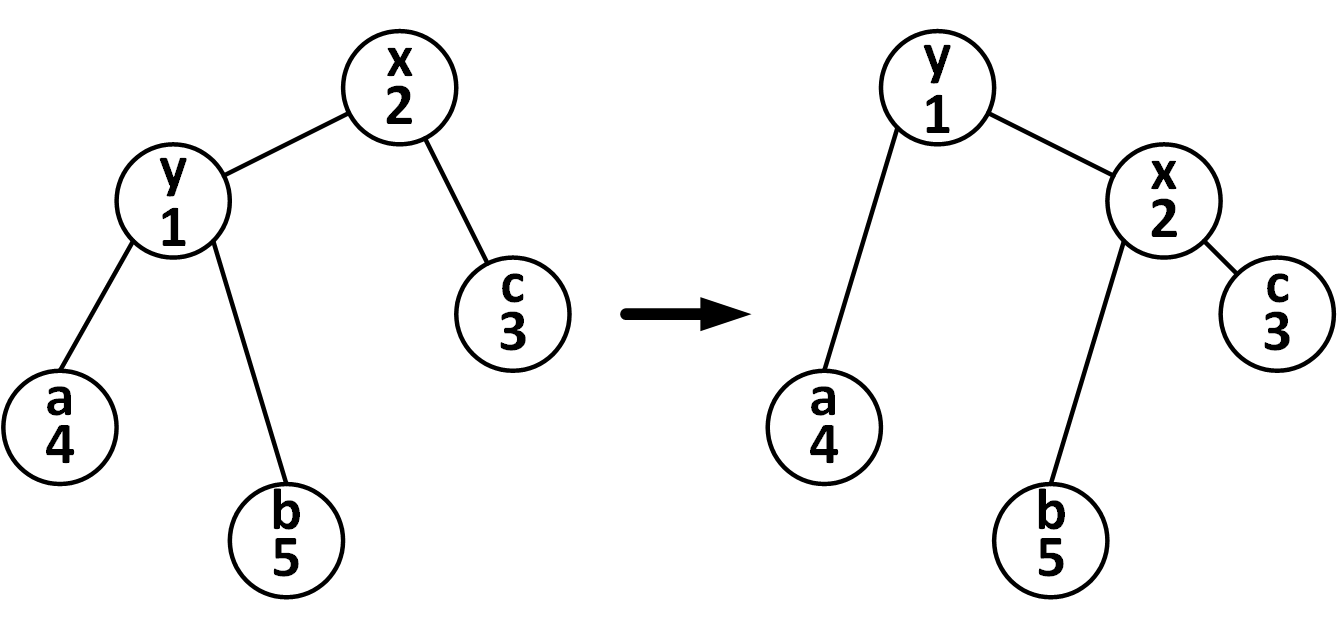
\includegraphics[width=0.7\textwidth,center]{fig/6-7.png}
    \end{itemize}
\end{frame}
\begin{frame}{3481 -- Double Queue (poj.org)}
    \begin{itemize}
        \item  系统为客户服务,每个客户有一个标识$k$,一个优先级$p$。这个系统可以接收的请求和对应的策略如下:
    \end{itemize}
    \begin{table}
        \begin{tabular}{l|l}
            请求      & 策略                               \\\hline
			 0         & 停止服务                          \\\hline
			 1 $k$ $p$ & 添加优先级$p$的客户$k$             \\\hline
			 2         & 服务优先级最高的客户并移除等待队列 \\\hline
			 3         & 服务优先级最低的客户并移除等待队列 \\\hline
        \end{tabular}
    \end{table}
\end{frame}
\begin{frame}{6.5 哈希表}
    \begin{block}{散列表}
        散列表(Hash table,也叫哈希表)基本原理是使用一个下标范围比较大的数组$H[1\ldots m]$来存储元素$x$
    \end{block}    
    \begin{itemize}
        \item 设计一个哈希函数,使得每个$x$都与一个函数值$y$(即数组$H$的下标)相对应,然后用$H[y]$指向元素$x$,没有元素指向,则$H[y]=\phi$
        \item 由于不能够保证每个元素的关键字与函数值是一一对应的,因此很有可能出现如下情况:对于不同的元素$x_1,x_2$,哈希函数计算出了相同的函数值$y$,这就是产生了所谓的\textcolor{red}{“冲突”},换句话说,就是哈希函数同一个$H[y]$指向了不同的元素$x_1,x_2$
        \item 常用的字符串哈希函数有BKDRHash、PJWHash(ELFHash)、APHash等,效率较高的为BKDRHash函数\footnote{\url{https://byvoid.com/zhs/blog/string-hash-compare/}}
    \end{itemize}
\end{frame}
\begin{frame}{解决冲突}
\begin{enumerate}
    \item \textcolor{blue}{链接表},将相同函数值的所有元素放在一个链表中,$H[y]$指向这个链表
    \item \textcolor{blue}{开放寻址法}
    \begin{itemize}
        \item 最简单的是线性探测再散列技术,即当$H[y]\neq\phi$,说明$H[y]$位置已经存储有元素,依次探测$(y+i)\mod m, i=1,2,3\ldots$,直到找到空的存储单元为止
        \item 当冲突严重时,扫描到空单元的时间会变长,哈希表越满,这种情况带来时间消耗就会越大,这时通过扩大数组范围$m$可以有效减少查找时间
        \item 设计一个好的哈希函数是解题的关键,而实际应用中,哈希函数的种类很多,可以应用到多个领域 ,理解哈希函数的作用十分必要
    \end{itemize}
\end{enumerate}
\end{frame}
\begin{frame}{2503 -- Babelfish (poj.org)}
    \begin{itemize}
        \item 给出字典条目分为<英语 外语>,接下来给出外语,在字典中查找对应的英语并输出,如果查不到,输出“eh”
        \item 采用哈希表解决,将字符串转换成对应的哈希值,这样在查找时会提高效率
        \item 将外语词条保存到一个哈希表$H$中,英语保存到对应的表$A$中
        \begin{enumerate}[(1)]
            \item \textcolor{blue}{向哈希表添加元素}:通过一个字符串哈希函数将外语字符串$x$转化成整数$y$,将$x$保存到$H[y]$中,将$x$对应的英语保存到$A[y]$中。如果冲突,按照线性探测再散列的方法,令$y=y+i(i=1,2,\ldots )$
            \item \textcolor{blue}{在哈希表中查找元素}:当需要查找外语字符串$x$,先通过哈希函数计算出$x$的哈希值$y$,读出$H[y]$的值,将$H[y]$和$x$比较,如果相等,则对应的$A[y]$就是要求的内容;如果不相等,说明之前$H[y]$发生冲突,存储了其他的字符串的位置,这时需要在$y+i(i=1,2,\ldots )$位置继续查询;$H[y]=\phi$表明没有找到
        \end{enumerate}
        \item 越接近单词总量,哈希表剩余的空位置越少,由于查找是到下一个空位置终止,终止前花费的查找时间就会越长
    \end{itemize}
\end{frame}
\begin{frame}{6.6 字符串}
    \begin{itemize}
        \item 字符串一个常见的应用就是\textcolor{blue}{模式匹配}问题,比如文本编辑软件中的查找功能,网页搜索,GNU的grep命令等
        \vfill
        \item 将字符串扩展到大量的文本,需要更高效的数据结构和算法来实现
        \vfill
        \item 除了\textcolor{blue}{Trie树}、\textcolor{blue}{KMP算法}之外,还有\textcolor{blue}{后缀树}(Suffix tree) ,\textcolor{blue}{后缀数组}(Suffix array) ,\textcolor{blue}{Boyer-Moore字符串搜索算法}, 在文本里搜索多个字符串的\textcolor{blue}{Aho-Corasick算法}(AC自动机)等
    \end{itemize}
\end{frame}
\begin{frame}{字典树}
    \begin{itemize}
        \item \textcolor{blue}{Trie树},也称前缀树或字典树
        \begin{itemize}
            \item 例如:"a", "to", "tea", "ted", "ten", "i", "in", "inn"构成的trie树如图所示。根节点为空字符串, 每个字符串从根节点到对应的叶子节点,每个节点的子孙都有相同的前缀
            \item trie树使用链表存储,也可以使用二维数组,二维数组在空间上有所浪费,但是建树和查找过程效率很高
        \end{itemize}
    \end{itemize}    
    \begin{center}
        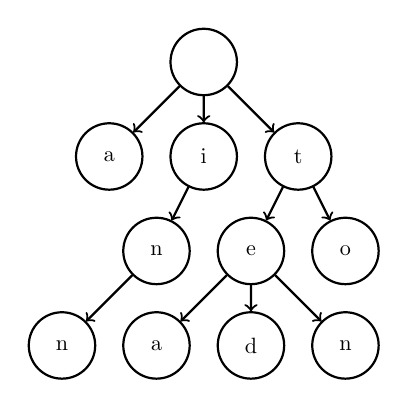
\begin{tikzpicture}
        [every node/.style={circle,minimum width=30pt,minimum height=30pt,thick,draw},
        edge from parent/.style={->,thick,draw},global scale=0.8]
        \node{}
        child{node{a}}
        child{node{i}
            child{node{n}
                child{node{n}}
                child[missing]{}
                child[missing]{}}
            child[missing]{}}
        child{node{t}
            child{node{e}
                child{node{a}}
                child{node{d}}
                child{node{n}}}
            child{node{o}}};
        \end{tikzpicture}  
    \end{center}
\end{frame}
\begin{frame}{字典树}
    \begin{itemize}
        \item 使用二维数组建树后的内容如图所示。数组trie[i,j]中存储的值为字符插入树的顺序pos,从根节点到pos的路径就是pos后面包含字符串的公共前缀; 图中数字上标为数组num[pos],其值为多少字符串以根到pos为前缀
    \end{itemize}
    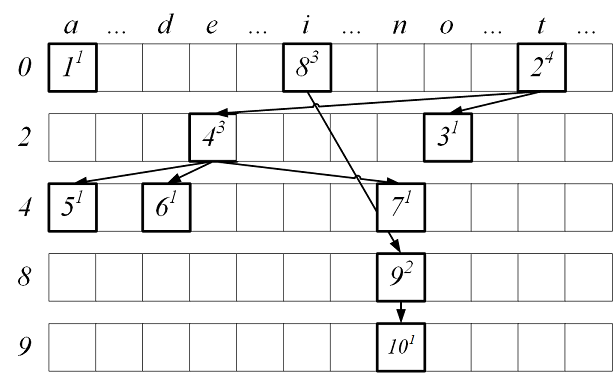
\includegraphics[width=0.7\textwidth,center]{fig/6-9.png}
\end{frame}
\begin{frame}{2001 -- Shortest Prefixes (poj.org)}
    \begin{itemize}
        \item A \textcolor{blue}{prefix} of a string is a substring starting at the beginning of the given string. The prefixes of "carbon" are: "c", "ca", "car", "carb", "carbo", and "carbon". Note that the empty string is not considered a prefix in this problem, but every non-empty string is considered to be a prefix of itself.
        \item In everyday language, we tend to abbreviate words by prefixes. For example, "carbohydrate" is commonly abbreviated by "carb".
        \item In this problem, given a set of words, you will find for each word the shortest prefix that uniquely identifies the word it represents.
    \end{itemize}
\end{frame}
\begin{frame}{3461 -- Oulipo (poj.org)}
    \begin{itemize}
        \item 题意:给出字符串W和T,求W在T中出现的次数
        \item Knuth-Morris-Pratt字符串查找算法(\textcolor{blue}{KMP算法}) :基于前缀匹配的方法,可以提高匹配效率
        \item 如图所示,当P[6]≠S[6]时,可以退回到P[2]继续匹配,用一个数组next记录回退的位置,比如next[6]=2,就可以通过该数组实现回退
        \item next数组的求法相当于在P数组内部进行字符串的匹配,值就是匹配到的共同前缀长度
    \end{itemize}
    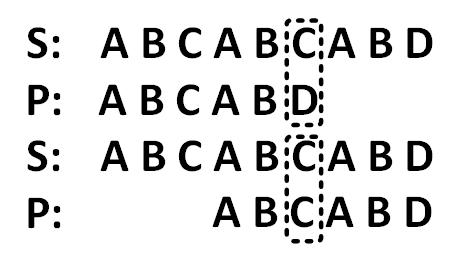
\includegraphics[width=0.5\textwidth,center]{fig/6-10.png}
\end{frame}
\end{document}